\chapter{Hajautettu järjestelmä}
\label{ch:distributed-systems}
% TODO: Kun tämän osion on kokonaan kirjoittanut niin siivoa tämä vastaamaan sitä.
Tässä osiossa käydään läpi järjestelmän hajauttamisen liityviä asioita, kuten mikä on hajautettu järjestelmä ja sen eri paradigmoja. Paradigmoista toteutetaan analyysi ja niistä arvioidaan niiden hyviä ja huonoja puolia. Lopuksi käsitellään avointa AMQP-standardia (engl. \emph{Advanced Message Queuing Protocol}) ja mitä hajautuksen paradigmoja se mahdollistaa.


\section{Mikä on hajautettu järjestelmä?}
\emph{Hajautettu järjestelmä} (engl. \emph{distributed system}) on verkko toisiinsa kytkettyjä fyysisiä- tai ohjelmistopohjaisia komponentteja, jotka kommunikoivat toistensa kanssa viestien välityksellä. Hajautetussa järjestelmässä osapuolten etäisyydellä ei ole merkitystä. Niiden välimatka voi olla eri maa tai sama rakennus. Hajautetut järjestelmät ovat oma tieteenala joka lähti liikkeelle käyttöjärjestelmien arkkitehtuurien tutkimuksista 1960-luvulla \cite[s.~384]{andrews2000foundations}. Ensimmäinen laajalle levinnyt hajautettu järjestelmä oli lähiverkot (engl. Local Area Network tai LAN), joka keksittiin 1970-luvulla \cite[s.~32]{andrews2000foundations}. Hajautetun järjestelmän määrityksistä ja toteuttamisesta on nykypäivänä olemassa hyvin kirjallisuutta ja tietoa, esimerkiksi \cite{distributed-systems-concepts-and-design, distributed-event-based-systems, mullender1993distributed, baldoni2005distributed}.

Järjestelmän hajautuksessa ja sen käytössä on pääasiassa kyse resurssien jakamisesta osapuolien kesken. Resurssi on abstrakti käsite ja voi tarkoittaa tekniikasta tai toteutuksesta riippuen montaa eri asiaa. Resurssilla voidaan esimerkiksi kuvata jaettua fyysistä laitetta kyten levyä tai tulostinta, ohjelmiston tapauksessa oliota tai tietokantaa \cite[s.~2--3]{distributed-systems-concepts-and-design}. Nykyinen internet mahdollistaa monien eri laitteiden kytkemisen verkkoon ja niiden kommunikoinnin keskenään, ja on nykypäivänä hyvä esimerkki todella laajasta hajautetusta järjestelmästä.

Hajautetussa järjestelmässä voidaan puhua osapuolten \emph{heterogeenisyydestä} (engl. \emph{heterogeneity}), eli osapuolet voivat kommunikoida toistensa kanssa tekniikasta tai toteutuksesta riippumatta. Tämä voidaan kuvata kerrosarkkitehruurin avulla. Korkean ja matalan tason ohjelmistojen välissä on ns. \emph{väliohjelmistokerros} (engl. \emph{middleware}). Tämän kerroksen tehtävä on abstrahoida matalan tason ohjelmisto tai alusta ja tehdä siitä heterogeeninen ylemmän tason ohjelmistoille ja palveluille. Kuvassa \ref{fig:middleware-architecture} on esitetty edelle mainittu kerrosarkkitehtuuri. \mbox{\cite[s. ~16--17]{distributed-systems-concepts-and-design}} \mbox{\cite[s.~2--3]{distributed-event-based-systems}}

\begin{figure}[ht!]
	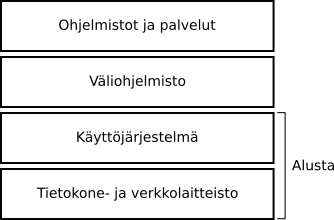
\includegraphics[width=0.5\textwidth]{pictures/middleware-architecture.png}
	\caption{Väliohjelmistokerros abstrahoimaan alusta heterogeeniseksi ylemmän tason ohjelmistolle (pohjautuu kuvaan \mbox{\cite[s.~52]{distributed-systems-concepts-and-design}}).}
	\label{fig:middleware-architecture}
\end{figure}


\subsection{Kuinka osapuolet kommunikoivat?}
Hajautetussa järjestelmässä osapuolet kommunikoivat keskenään viestien välityksellä. Jotta viestit voitaisiin vaihtaa tekniikasta riippumattomasti osapuolten välillä, täytyy tieto esittää alustariippumattomassa muodossa. Kommunikoivien osapuolten täytyy sopia yhteisestä viestin formaatista. Ohjelmat yleensä käsittelevät tietoa ohjelmistokielen tarjoamilla tietorakenteilla kuten esimerkiksi listoilla, puurakenteilla ja luokilla. Jotta tieto saadaan lähetettyä viestinä, täytyy se ensin muuntaa lähetykseen sopivaan muotoon. Tämä prosessi tunnetaan englannin kielellä nimellä \emph{marshalling}. Jotta vastaanotettua tietoa voidaa käyttää, täytyy viesti purkaa takaisin ohjelmistokielen rakenteiksi. Tämä prosessi englannin kielessä tunnetaan nimellä \emph{unmarshalling}. \mbox{\cite[s.~158]{distributed-systems-concepts-and-design}}

Kommunikointiin voidaan osapuolten välillä sopia erilaisista takuita lähetyksistä ja tiedon oikeudesta. Lähettäjä voi esimerkiksi vaatia vastaanottajaa kuittaamaan viestin vastaanottamisen. Jos kuittausta ei tule tietyn ajan sisällä, lähettäjä uudelleenlähettää viestin vastaanottajalle. Esimerkki tästä on TCP-protokollan (engl. Transmission Control Protocol) paketit, jossa lähettäjä odottaa vastaanottajan kuittausta paketista \cite[s.~9--10]{tcp-standard}. On myös tilanteita jossa lähettäjä ei välitä saako vastaanottaja viestin. Tässä tapauksessa osapuoli lähettää viestejä ilman tietoa siitä ottaako niitä kukaan vastaan. Esimerkki tästä on UDP-prokollan (User Datagram Protocol) paketit jossa lähettäjä ei odota kuittausta paketteihin \cite{udp-standard}. Uuden onnistuneesti lähetetyn paketin odotetaan korvaavan entisen tieto. Minkälainen takuu viestien lähetykseen valitaan riippu ohjelmiston vaatimuksista.


\subsection{Kommunikoinnin luokittelu}
Hajautetuissa järjestelmissä osapuolten kommunikoinnin välillä voi olla \emph{suora-} tai \emph{epäsuora liitos}. Suora liitos tarkoittaa tilannetta, jossa osapuolet tietävät toistensa identiteetin. Esimerkiksi lähettäjä lähettää viestiin suoraan vastaanottajalle. Epäsuora liitos tilannetta jossa osapuolet eivät tiedä toistensa identiteettiä. Epäsuorassa liitoksessa osapuolet yleensä kommunikoivat välittäjän kautta, joka hoitaa viestien lähettämisen toiselle osapuolelle. Suorassa liitoksessa toisen osapuolen vaihtaminen on vaikeampaa kuin epäsuorassa liitoksessa. Esimerkkinä tästä on yksinkertainen asiakas-palvelin-malli. Suoran liitoksen takia palvelin on vaikeampi vaihtaa toiseen samanlaiseen (palvelin tulkkaa HTML-sivuja asiakkalle). Epäsuorassa liitoksessa palvelimen vaihto samanlaiseen on helpompaa jos niiden välissä on tarpeeksi epäsuoruutta (geneerinen rajapinta tai välittäjä). \cite[s.~230]{distributed-systems-concepts-and-design}

Hajautetuissa järjestelmissä voidaan puhua erilaisista heikkojen liitoksien luokittelumalleista. Kirjallisuudessa näitä kutsutaan
\begin{itemize}
	\item \emph{heikko tilaliitos} (engl. \emph{space uncoupling}), tarkoittaa liitosta jossa osapuolet eivät tiedä toistensa identiteettiä, ja
	\item \emph{heikko aikaliitos} (engl. \emph{time uncoupling}), tarkoittaa liitosta jossa osapuolien ei tarvitse olla olemassa samaan aikaan.
\end{itemize}
Näiden mukaan voidaan esittää malli, jolla luokitellaan osapuolten välistä liitosta. Tämä malli on esitetty taulukossa \ref{tab:communication-models}. \cite[s.~230]{distributed-systems-concepts-and-design} \cite[s.~116]{eugster2003many}

\begin{table}[ht!]
	\caption{Hajautetussa järjestelmässä osapuolten kommunikoinnin luokittelun malli (pohjautuu taulukoihin \mbox{\cite[s.~231]{distributed-systems-concepts-and-design}} \mbox{\cite[s.~84]{cabri2000mobile}}).}
	\label{tab:communication-models}
	\begin{tabular}{p{0.1\linewidth} | p{0.37\linewidth} | p{0.37\linewidth}}
		\hline
		& \textbf{Vahva aikaliitos} & \textbf{Heikko aikaliitos} \\
		\hline
		\textbf{Vahva tilaliitos} & Kommunikointi tarkoitettu suoraan toiselle osapuolelle. Osapuolten täytyy olla olemassa samaan aikaan, esimerkiksi suora viestintä tai etäfunktiokutsu. & Kommunikointi tarkoitettu suoraan toiselle osapuolelle. Osapuolet voivat olla olemassa eri aikaan.\\
		\hline
		\textbf{Heikko tilaliitos} & Osapuolten ei tarvitse tietää toistensa identiteettiä. Osapuolten täytyy olla olemassa samaan aikaan, esimerkiksi IP-ryhmälähetys. & Osapuolten ei tarvitse tietää toistensa identiteettiä. Osapuolet voivat olla olemassa eri aikaan, esimerkiksi tilaaja-julkaisija-malli ja viestijono \\
		\hline
	\end{tabular}
\end{table}

Taulukossa \ref{tab:communication-models} vasemmassa yläkulman luokittelu tarkoittaa kommunikointia, missä osapuolet tietävät toistensa identiteetin ja niiden täytyy olla olemassa samaan aikaan. Tämä on siis kaikista vahvin liitos mitä osapuolten välillä voi olla ja jossa on vähiten epäsuoruutta. Esimerkkinä tästä kommunikoinnista on etäfunktiokutsu tai suora viestintä prosesseiden välillä. Oikeassa yläkulmassa on tilanne, jossa osapuolet edelleen tietävät toistensa identiteetin, mutta niiden ei tarvitse olla olemassa samaan aikaan. Esimerkkinä osapuoli lähettää viestin tietylle identiteetille, mutta vastaanottaja ottaa viestin vastaan vasta myöhemmin. Teknistä esimerkkiä tähän tilanteeseen on hankalampi esittää kuin taulukon muihin kohtiin. Taulukon vasemmassa alakulmassa on tilanne jossa osapuolet eivät teidä toistensa identiteettiä, mutta niiden täytyy olla olemasa samaan aikaan. Esimerkkinä tästä on IP-ryhmälähetys, jossa viesti lähetetään kaikille verkon osapuolille ilman tietoa niiden identiteetistä. Vastaanottaja on olemassa samaan aikaan ja vastaa lähettäjälle ilman identiteettiä. Taulukon oikeassa alakulmassa on tilanne missä osapuolten välillä on kaikista eniten epäsuoruutta muista luokitteluista. Osapuolet eivät tiedä toistensa identiteettiä ja niiden ei tarvitse olla olemassa samaan aikaan. Esimerkkinä tilaaja-julkaisija- ja viestijono-mallit. \mbox{\cite[s.~230--232]{distributed-systems-concepts-and-design}} \mbox{\cite{cabri2000mobile}}

Epäsuoruus ohjelmoinnissa tuo hyötyjä ja joustavuutta ohjelmaan ja sen toimintaa kuten aikaisemmin tuotiin esille. Epäsuoruuden mukana tulee myös haittoja, kuten kommunikointi voi olla vaikeampaa osapuolten välillä ja epäsuoruus yleensä heikentää ohjelman suorituskykyä. Suorituskyky ja kommunikoinnin vaikeidet vaihtelevat tekniikasta ja toteutuksesta riippuen.

\section{Hajautuksen paradigmoja}
\begin{it}
	Kirjoita tähän asiaa paradigmoista ja vertaile niitä keskenään. Kerro mihin tilanteisiin se sopii ja sen huonot ja hyvät puolet.
	
	% TODO: Tästä kappaleesta lisää lyhenteet alkuun kun kirjoitus on tehty.
\end{it}

\begin{table}[ht!]
	\caption{Hajautetun järjestelmän kommunikointiparadigmat kolmella päätasolla (pohjautuu tauluun \mbox{\cite[s.~46]{distributed-systems-concepts-and-design}}).}
	\label{tab:communication-paradigms}
	\begin{tabular}{p{0.3\linewidth} | p{0.3\linewidth} | p{0.3\linewidth}}
		\hline
		\textbf{Prosessien välinen kommunikaatio} & \textbf{Etäkutsu} & \textbf{Epäsuora kommunikaatio} \\
		\hline \hline
		Viestien välitys (message passing) & Pyyntö-vastaus (request-reply) & Joukkokommunikointi (group communication) \\
		\hline
		Soketti (socket) & Etäproseduurikutsu (RPC) & Julkaisija-tilaaja (publish-subscribe) \\
		\hline
		Ryhmäkutsu (multicast) & Etämetodikutsu (RMI) & Viestijono (message queue) \\
		\hline
		& & Jonotaulu (tuple space) \\
		\hline
		& & Hajautetusti jaettu muisti (DSM) \\
		\hline
	\end{tabular}
\end{table}


\subsection{Julkaisija-tilaaja (publish-subscribe)}


\subsection{Viestijono (message queue)}


\subsection{Pyyntö-vastaus (request-reply)}


\section{Advanced Message Queuing Protocol (AMQP)}
\label{ch:amqp-theory}
Työssä toteutettu ohjelmisto tilasi viestit IED-laitteen RCB-instansseilta. Viestit tilattiin verkon yli aseman ulkopuolelle. Ohjelma prosessoi IEC 61850 -standardin mukaiset viestit ja lähetti ne eteenpäin välittäjälle (engl. message broker). Välittäjä on verkossa oleva erillinen palvelin, mistä muut ohjelmat pystyvät tilaamaan viestejä tarpeidensa mukaan. Kuvassa \ref{fig:implemented-system-communication} on esitetty lopullisen toteutuksen tietoliikenne eri osapuolten välillä. Tässä työssä toteutettu ohjelmisto on merkitty kuvaan katkoviivalla. Toteutuksessa oli kyse tilaaja-julkaisija-arkkitehtuurimallista (engl. publish-subscribe pattern), jossa toteutettu komponentti oli tilaaja IED-laitteelle ja julkaisija välityspalvelimelle. Järjestelmän muut komponentit olivat tilaajia välityspalvelimelle. Tässä osuudessa perehdytään viestien välittäjän teoriaan, ja mitä siitä täytyy tietää ohjelmistokehityksen kannalta.

\begin{figure}[ht!]
	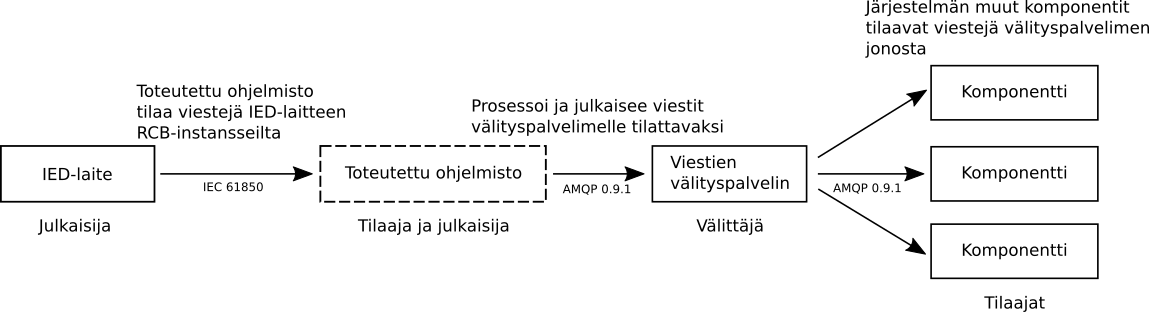
\includegraphics[width=1\textwidth]{pictures/implemented-system-communication.png}
	\caption{Toteutetun ohjelmiston osuus ja rooli kokonaisuudessa tietoliikenteen kannalta.}
	\label{fig:implemented-system-communication}
\end{figure}

Työssä välittäjänä käytettiin \emph{RabbitMQ}-ohjelmistoa \cite{rabbitmq-homepage}, joka on avoimen lähdekoodin välittäjäpalvelin ja perustuu avoimeen \emph{AMQP}-standardiin \cite{amqp-homepage} (engl. \emph{Advanced Message Queuing Protocol}). AMQP määrittää yhteisen protokollan viestintään eri ohjelmistojen välillä verkon yli välityspalvelimen avulla. Verkon ansiosta välityspalvelin voi sijaita eri koneella kuin sitä käyttävät ohjelmistot. Standarista on julkaistu monta eri versiota, ja työn tekohetkellä viimeisin versio oli 1.0. Kuitenkin RabbitMQ-ohjelmisto oli suunniteltu käytettäväksi standardin version 0.9.1 kanssa, ilman asennettuja lisäosia. Versioiden välinen ero oli suuri ja siirto uuteen ei ollut mahdollista, koska standardin versiot eivät olleet keskenään yhteensopivat. RabbitMQ tuki versiota 0.9.1 ja sen kehittäjät mieltävät standardin version 1.0 kokonaan eri protokollaksi \mbox{\cite{RabbitMQ-Compatibility-and-Conformance}}. Kuvassa \ref{fig:implemented-system-communication} on tietoliikenteen kohtiin merkitty mikä standardi vaikuttaa minkäkin osapuolen kommunikointiin. Tässä työssä välityspalvelin ja siihen yhteydessä olevat ohjelmistot käyttävät AMQP-standardista versiota 0.9.1.


\subsection{Advanced Message Queuing -malli ja sen osat}
AMQP-standardi määrittää komponentteja, joiden läpi viestin täytyy kulkea julkaisijalta tilaajalle. Standardissa nämä komponentit määrittää \emph{AMQ-malli} (engl. \emph{AMQ-model}). Kuvassa \ref{fig:amq-model-parts} on esitetty viestin kulku julkaisijalta tilaajalle mallin eri komponenttien läpi. Mallin komponentit ovat \emph{vaihde} (engl. \emph{exchange}), \emph{jono} (engl. \emph{queue}) ja näiden välinen \emph{sidonta} (engl. \emph{binding}). Välityspalvelimen tehtävän voi tiivistää niin, että se ottaa vastaan viestejä julkaisijoilta vaihteeseen. Vaihde reitittää viestejä tilaajille jonoihin määritettyjen sidosten mukaan. Jos tilaaja ei ehdi prosessoida viestejä tarpeeksi nopeasti, palvelin pitää viestit jonossa tilaajalle. Vaihde voi välittää viestin moneen eri jonoon ja yhtä jonoa voi tilata monta eri asiakasta.

\begin{figure}[ht!]
	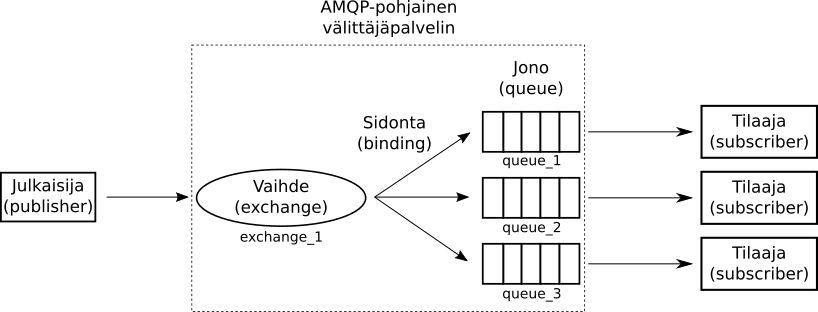
\includegraphics[width=1\textwidth]{pictures/amq-model-parts.png}
	\caption{AMQ-mallin osat ja viestin kulku niiden läpi julkaisijalta tilaajalle (pohjautuu kuvaan \mbox{\cite[s.~11]{AMQP-specification}}).}
	\label{fig:amq-model-parts}
\end{figure}

AMQP on ohjelmoitava protokolla siinä mielessä, että julkaisija ja tilaaja voivat määrittää komponentteja ja reitityksiä palvelimelle verkon yli ajon aikana tarpeidensa mukaan. Välittäjäpalvelin ei määritä kuin oletusvaihteet valmiiksi käytettäväksi. Toisin sanoen julkaisuja voi luoda vaihteita ja tilaaja voi luoda jonoja ja sidoksia vaihteiden ja jonojen välille. Voidaan sanoa että julkaisija ja tilaaja tekevät uusia instansseja AMQ-mallin komponenteista palvelimelle. Vaihteiden ja jonojen instansseilla täytyy olla välityspalvelimella yksilöivät nimet, jokainen nimi asetetaan instanssin luonnin yhteydessä. Esimerkkinä kuvassa \ref{fig:amq-model-parts} on AMQ-mallin komponenttien alla niille määritetyt nimet. Vaihteella on esimerkiksi nimi exchange\_1 ja ylimmällä jonolla queue\_1. Tällä ohjelmoitavalla ominaisuudella välityspalvelin voidaan konfiguroida toteuttamaan erilaisia skenaarioita vapaasti ja se antaa kehittäjille vapautta toteutukseen.


\subsection{Vaihde (exchange) ja reititysavain (routing-key)}
Jotta viesti voidaan kuljettaa välittäjäpalvelimen läpi, täytyy julkaisijan aloittaa määrittämällä käytetty vaihde ja sen tyyppi. Julkaisija voi myös käyttää palvelimen oletusvaihdetta. Vaihde on komponentti, joka ottaa vastaan viestejä ja reitittää niitä jonoihin vaihdetyypin (engl. exchange type) ja sidosten mukaan. Vaihteet eivät ikinä tallenna viestejä. Vaihde voi tiputtaa viestin, jos se ei täsmää minkään määritetyn reitityksen kanssa. AMQ-malli määrittää seuraavat käytettävät vaihdetyypit:
\begin{itemize}
	\item \emph{suoravaihde} (engl. \emph{direct exchange}),
	\item \emph{hajautusvaihde} (engl. \emph{fanout exchange}), ja
	\item \emph{aihepiirivaihde} (engl. \emph{topic exchange}).
\end{itemize}

Näitä tyyppejä ja kuinka ne toimivat käydään tarkemmin läpi tulevissa kappaleissa. Tyypin lisäksi vaihteella on myös attribuutteina \emph{nimi} (engl. \emph{name}), \emph{kestävyys} (engl. \emph{durability}), \emph{automaattinen poisto} (engl. \emph{auto-delete}). Nimi yksilöi vaihteen palvelimella ja tilaaja käyttää tätä nimeä sidoksen tekemiseen jonon ja vaihteen välille. AMPQ-standardissa oletetaan, että nimi on jo tiedossa etukäteen julkaisijalla ja tilaajalla. AMPQ ei tarjoa toiminnallisuutta instanssien nimien noutamiseen. Kestävyys parametrilla julkaisija voi kertoa palvelimelle, että välitäjä säilyttää vaihteen uudelleenkäynnistysten jälkeen. Jos ei, julkaisijan täytyy määrittää vaihde uudelleen käynnistyksen jälkeen. Automaattinen poisto kertoo poistaako välittäjä vaihteen automaattisesti, kun viimeinen siihen sidottu jono on poistettu ja julkaisija ei ole enää yhteydessä.

Kaikki julkaisijan ja tilaajan kutsut välittäjäpalvelimelle, jotka tekevät uuden instanssin komponentista, ovat esitteleviä (engl. declare). Tämä tarkoittaa että palvelin tekee tarvittaessa uuden instanssin komponentista, jos sitä ei ole jo olemassa ja vastaa onnistuneesti molemmissa tapauksissa. Tilanne tulee esimerkiksi silloin kun kaksi julkaisijaa käyttävät samaa vaihdetta keskenään. Toinen ei tiedä onko toinen jo määrittänyt instanssin vaihteesta palvelimelle, esimerkiksi silloin kun ohjelmat käynnistyvät eri aikaan. Jos kummatkin julkaisijat eksplisiittisesti määrittävät saman käytettävän vaihteen. Palvelin vastaa kummallekin onnistuneesti ja tuloksena palvelimella on vain yksi instanssi halutusta vaihteesta. Sama toiminta pätee kaikkiin välittäjäpalvelimen kutsuihin, jotka tekevät uusia instansseja komponenteista.

Vaihde reitittää viestejä jonoihin sen sidosten ja tyypin mukaan. Reititykseen liittyy tärkeä asia, joka on \emph{reititysavain} (engl. \emph{routing-key}). Reititysavain on kuin virtuaalinen osoite viestissä, jonka julkaisija liittää viestiin julkaisun yhteydessä. Tilaaja käyttää myös reititysavainta jonon määrityksen yhteydessä. Vaihde, tyypistä riippuen, voi käyttää tätä avainta reititykseen eri jonoihin. Viestin reititysavainta voi hyvin verrata lähetettävän sähköpostin saaja-kenttään. Saaja kertoo vastaanottajan sähköpostiosoitteen, johon viesti on tarkoitus lähettää. Reititysavain toimii juurikin näin suorassa viestin lähetyksessä, mutta eroaa muissa.


\subsection{Suoravaihde (direct exchange)}
\label{ch:direct-exchange}
Julkaisija voi määrittää vaihteen instanssin tyypiksi suoravaihteen (engl. direct exchange). Suoravaihde reitittää viestin jonoihin vastaavan reititysavaimen perusteella. Suoravaihde reitittää seuraavasti:
\begin{itemize}
	\item tilaaja määrittää sidoksen reititysavaimella K,
	\item julkaisija julkaisee viestin reititysavaimella R,
	\item vaihde välittää viestin jonoon jos K = R,
	\item muuten vaihde tiputtaa tai palauttaa viestin lähettäjälle.
\end{itemize}
Kuvassa \ref{fig:amqp-direct-exchange} on esitetty suoravaihteen toiminta. Vaihteeseen on tehty sidoksia reititysavaimilla error ja info. Yksi tilaaja voi luoda sidoksia samaan vaihteeseen monella eri reititysavaimella. Näin tilaaja voi tilata viestejä mistä on kiinnostunut. Kuvassa \ref{fig:amqp-direct-exchange} julkaisija julkaisee viestin reititysavaimella info. Viesti päätyy molempiin queue\_1 ja queue\_2 jonoon. Reititysavaimella error, viestit päätyvät vain jonoon queue\_1. Välittäjäpalvelin tarjoaa suoravaihteesta oletusvaihteen nimeltä \emph{amq.direct}. \mbox{\cite[s.~27]{AMQP-specification}}

\begin{figure}[ht!]
	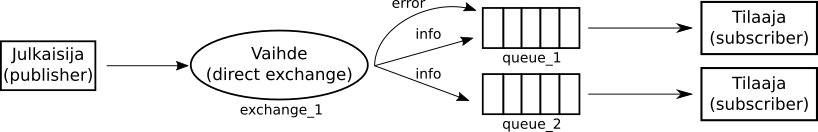
\includegraphics[width=1\textwidth]{pictures/amqp-direct-exchange.png}
	\caption{Suoravaihde (engl. direct exchange), reitittää suoraan sidoksen reititysavaimen mukaan (pohjautuu kuvaan \mbox{\cite{RabbitMQ-Tutorial-Routing}}).}
	\label{fig:amqp-direct-exchange}
\end{figure}


\subsection{Hajautusvaihde (fanout exchange)}
Julkaisija voi määrittää vaihteen instanssiksi hajautusvaihteen (engl. fanout exchange). Hajatusvaihde reitittää viestit kaikkiin sen jonoihin reititysavaimesta välittämättä. Hajautusvaihde toimii seuraavasti:
\begin{itemize}
	\item tilaaja määrittää sidoksen vaihteeseen reititysavaimella K,
	\item julkaisija julkaisee viestin reititysavaimella R,
	\item vaihde välittää viestin kaikkiin siihen sidottuihin jonoihin, reititysavaimesta riippumatta.
\end{itemize}
Kuvassa \ref{fig:amqp-fanout-exchange} on esitetty hajautusvaihteen toiminta. Vaihteeseen exchange\_1 on tehty kolme eri sidosta jonoihin queue\_1, queue\_2 ja queue\_3. Julkaisijan lähettämä viesti lähetetään kaikkiin kolmeen sidottuun jonoon, viestin ja jonojen reititysavaimista riippumatta. Välittäjäpalvelin tarjoaa hajautusvaihteesta oletusvaihteen nimeltä \emph{amq.fanout}. \mbox{\cite[s.~27]{AMQP-specification}}

\begin{figure}[ht!]
	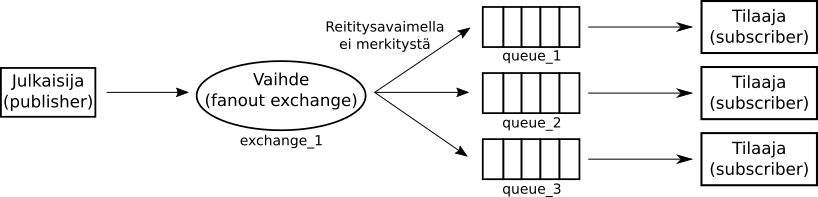
\includegraphics[width=1\textwidth]{pictures/amqp-fanout-exchange.png}
	\caption{Hajautusvaihde (engl. fanout exchange) reitittää kaikkiin siihen sidottuihin jonoihin riippumatta reititysavaimesta (pohjautuu kuvaan \mbox{\cite{RabbitMQ-AMQP-0-9-1-Model-Explained}}).}
	\label{fig:amqp-fanout-exchange}
\end{figure}


\subsection{Aihepiirivaihde (topic exchange)}
Aihepiiri-vaihdetyyppi (engl. topic exchange) reitittää viestejä sidottuihin jonoihin reititysavaimen mukaan kuin suoravaihde, mutta tarjoaa lisäksi sääntöjä monen avaimen samanaikaiseen yhteensopivuuteen. Sidoksen reititysavaimen sijaan voidaan puhua reitityskaavasta (engl. routing pattern). Aihepiiri vaihde toimii seuraavasti:
\begin{itemize}
	\item tilaaja määrittää sidoksen vaihteeseen reitityskaavalla P,
	\item julkaisija julkaisee viestin reititysavaimella R,
	\item vaihde välittää viestin jonoon, jos sen reitityskaava P sopii reititysavaimeen R.
\end{itemize}
Aihepiirivaihteessa reititysavaimen täytyy olla lista sanoja, jotka ovat erotettu pisteillä ja ovat yhdessä maksimissaan 255 merkkiä pitkä \mbox{\cite[s.~35]{AMQP-specification}}. Sanat saavat sisältää kirjaimia A-Z ja a-z, ja numeroita 0-9. Yleensä avaimeen sijoitetaan sanoja mitkä liittyvät viestin sisältöön. Tilaajan määrittämä sidoksen reitityskaava voi olla samaa muotoa kuin reititysavain, mutta sanojen tilalla voidaan käyttää seuraavia erikoismerkkejä:
\begin{itemize}
	\item \textbf{*} (tähti), voi vastata mitä tahansa yhtä sanaa,
	\item \textbf{\#} (risuaita), voi vastata nolla tai monta sanaa. \mbox{\cite[s.~27]{AMQP-specification}}
\end{itemize}

Kuvassa \ref{fig:amqp-topic-exchange} on esitetty aihepiirivaihteen toiminta. Vaihteeseen exchange\_1 on sidottu jono queue\_1 reitityskaavoilla \emph{app1.\#} ja \emph{*.*.warn}. Ja jono queue\_2 reitityskaavalla \emph{*.log.*}. Oletetaan, että julkaisija lähettää viestejä avaimella muodossa \emph{ohjelma.kanava.taso}, jossa \emph{ohjelma} kuvaa julkaisijan nimeä. \emph{Kanava} kuvaa lokitusväylää ja \emph{taso} kuvaa viestin tasoa (warning, error, info jne.). Voisi sanoa että queue\_1 on kiinnostunut kaikista ohjelmalta app1 tulevista viesteistä ja myös kaikista varoitustason (warning) viesteistä. Jono queue\_2 on vain kiinnostunut kaikista log-väylän viesteistä.

\begin{figure}[ht!]
	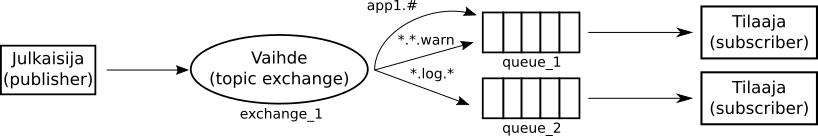
\includegraphics[width=1\textwidth]{pictures/amqp-topic-exchange.png}
	\caption{Aihepiirivaihde (engl. topic exchange), reitittää kaikkiin siihen sidottuihin jonoihin, joiden reitityskaava sopii viestin reititysavaimeen (pohjautuu kuvaan \mbox{\cite{RabbitMQ-Tutorial-Topics}}).}
	\label{fig:amqp-topic-exchange}
\end{figure}

Nyt jos julkaisija lähettää viestin avaimella \emph{app1.debug.warn}, vaihde välittää viestin jonoon queue\_1, mutta ei jonoon queue\_2. Avaimella \emph{app2.log.info} viesti välitetään vain jonoon queue\_2. Avaimella \emph{app1.log.warn} viesti lähetään molempiin jonoihin. Kun taas avaimella \emph{app2.debug.info} viestiä ei lähetetä yhteenkään jonoon.

Aihepiirivaihde on vaihdetyypeistä monimutkaisin, mutta kattaa ison määrän erilaisia käyttötapauksia. Vaihteen avulla tilaajat voivat tilata viestejä, joista ovat esimerkiksi kiinnostuneita. Aihepiirivaihdetta voi käyttää kuin aikaisempia vaihdetyyppejä. Jos jono sidotaan reitityskaavalla \#, se vastaanottaa kaikki viestit kyseiseltä vaihteelta ja käyttäytyy kuin hajautusvaihde. Jos jono sidotaan ilman merkkejä * ja \#, niin se käyttäytyy samalla tavalla kuin suoravaihde. \mbox{\cite{RabbitMQ-Tutorial-Topics}}


\subsection{Jonon määritys ja viestien kuittaaminen}
AMQ-mallissa jono (engl. queue) on vaihteen ja tilaajan välissä oleva puskuri (kuva \ref{fig:amq-model-parts}), joka tallentaa tilaajalle tulevia viestejä. Jono pitää viestejä jonossa tilaajalle, kunnes tämä ehtii prosessoida ne. Yksi jono voi puskuroida viestejä monelle eri tilaajalle. Jotta jonoon saapuu viestejä, täytyy tilaajan sitoa (engl. binding) jono palvelimella olemassa olevaan vaihteeseen. Tällä mekanismilla tilaaja voi valita mistä julkaisijasta on kiinnostunut. Tilaaja voi sitoa saman jonon moneen eri julkaisijaan. Tämä mahdollistaa viestien tilaamisen monelta eri vaihteelta. Sidos vaihteeseen tehdään vaihteen nimellä, eli tilaajan täytyy tietää vaihteen nimi etukäteen. Jonolla tilaaja voi määrittää attribuutteja. Jotkin attribuutit ovat samoja kuin vaihteella. Tilaaja voi määrittää jonolle \emph{nimen} (engl. \emph{name}), \emph{kestävyyden} (engl. \emph{durable}), \emph{poissulkevuuden} (engl. \emph{exclusive}) ja \emph{automaattisen poiston} (engl. \emph{auto-delete}). Nimi yksilöi jonon palvelimella. Tilaaja voi halutessaan pyytää palvelinta generoimaan yksilöivän nimen jonolle automaattisesti. Kestävyys-attribuutti säilyttää jonon palvelimella uudelleenkäynnistyksen jälkeen. Poissulkeva rajoittaa jonon vain yhdelle tilaajalle ja palvelin poistaa jonon kun yhteys tilaajaan katkeaa. Automaattinen poisto poistaa jonon palvelimelta automaattisesti kun yhteys viimeiseen tilaajan on katkennut. \mbox{\cite{RabbitMQ-AMQP-0-9-1-Model-Explained}}

Jos saman nimisen jonoon on liittynyt monta eri tilaajaa. Palvelin lähettää viestin jonosta vain yhdelle tilaajalle kerrallaan kiertovuorottelu (engl. round-robin) periaatteen mukaan. Sama viesti lähetetään ainoastaan toiselle tilaajalle jos se edelleenlähetetään virheen tai peruutuksen seurauksena \mbox{\cite[s.~11--12]{AMQP-specification}}. Tilaajan täytyy määrittää jonolle sen käyttämä viestin kuittaamisen (engl. acknowledge) malli ennen kuin jono poistaa viestin puskurista. Malleja on kaksi:
\begin{itemize}
	\item automaattinen, jolloin palvelin poistaa viestin jonosta heti kun se on lähetetty tilaajalle,
	\item eksplisiittinen, jolloin palvelin poistaa viestin, kun tilaaja on lähettänyt kuittauksen palvelimelle.
\end{itemize}
Tilaaja voi lähettää viestistä kuittauksen milloin vain prosessoinnin aikana. Heti kun viesti on vastaanotettu tai silloin kun viesti on prosessoitu. \mbox{\cite[s.~29]{AMQP-specification}}